\documentclass[10pt,twocolumn,letterpaper]{article}

\usepackage{cvpr}
\usepackage{times}
\usepackage{graphicx}
\usepackage{amsmath}
\usepackage{amssymb}
\usepackage{booktabs}
\usepackage{array}
\usepackage{enumitem}
\usepackage{tikz}
\usetikzlibrary{positioning, arrows.meta, shapes.geometric, calc, fit, backgrounds}
\usepackage[breaklinks=true,bookmarks=false]{hyperref}
\usepackage{microtype}
\usepackage{balance}
\usepackage{subcaption}
\usepackage{float}

\cvprfinalcopy
\addtolength{\topmargin}{-0.4in}
\def\cvprPaperID{****}
\setcounter{page}{1}

\raggedbottom

\begin{document}

\title{Drift or Return? Fuel-Optimal Recovery of Perturbed Along-Track\\Satellite Formations via Sequential Convex Programming}

\author{
\begin{tabular}{c}
Rahul Ayanampudi \\
AeroAstro Department \\
Stanford University \\
{\tt\small rayanam@stanford.edu} \\
\end{tabular}
\begin{tabular}{c}
Zeb Barry \\
AeroAstro Department \\
Stanford University \\
{\tt\small zebbarry@stanford.edu} \\
\end{tabular}
\begin{tabular}{c}
Julian Brown \\
AeroAstro Department \\
Stanford University \\
{\tt\small julianb@stanford.edu} \\
\end{tabular}
}

\twocolumn[
  \maketitle
  \begin{center}
    \resizebox{0.92\textwidth}{!}{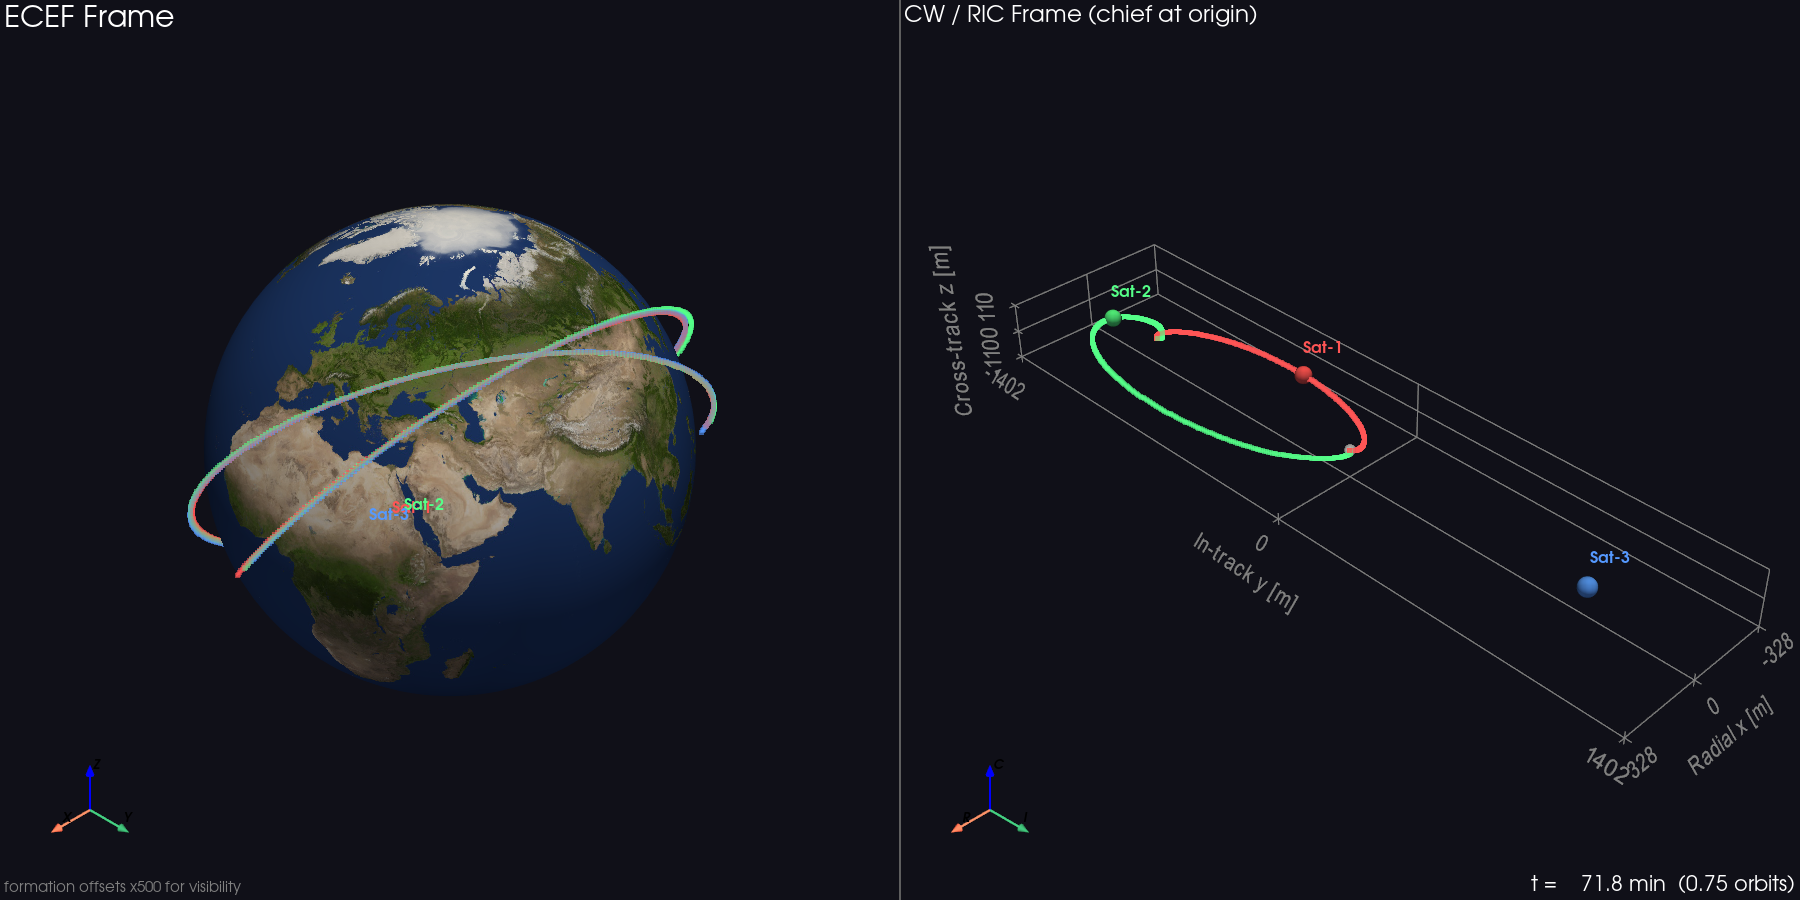
\includegraphics{figures/highlight_fig.png}}
    \vspace{0.35em}
    \captionof{figure}{\textbf{Dual-frame visualization of an SCP formation recovery.}
    \textbf{Left:} Earth-Centered Earth-Fixed (ECEF) view of the 550\,km, $51.6^\circ$
    chief reference orbit (a regressing spiral in the rotating frame) with the
    three labeled satellites; formation offsets are exaggerated $500\times$ so
    the satellites are individually visible at planetary scale. \textbf{Right:}
    Clohessy--Wiltshire (CW) / RIC view centered on the virtual chief: after an
    unexpected $\delta\mathbf{v}_0$ on Sat-2 (green), the SCP planner elects to
    \emph{swap} Sat-2 and Sat-1 (red) rather than fight the natural along-track
    drift, restoring the original 1\,km spacing for 0.30\,m/s of total $\Delta v$
    versus 2.27\,m/s for the return-to-slot baseline, while Sat-3 (blue) holds
    station. The simulator, solvers, and all figures are produced by our
    open Python package \texttt{cwsim}.}
    \label{fig:highlight}
  \end{center}
  \vspace{0.9em}
]

\begin{abstract}
Close-proximity satellite formations in Low Earth Orbit (LEO) operate with
narrow safety margins: a single unexpected velocity perturbation---a collision
avoidance burn or thruster misfire---induces secular along-track drift that
carries the perturbed satellite across the trajectories of its neighbors. We
ask whether the optimal response is to return the perturbed satellite to its
original slot, or to exploit the natural drift and re-order the formation. We
model a three-satellite along-track formation with the full
three-degree-of-freedom Clohessy--Wiltshire (CW) dynamics, propagated exactly
through the closed-form state transition matrix (STM), and compare two
recovery architectures: \textbf{(a)} a closed-form two-impulse CW solver that
restores the perturbed satellite to its original slot, and \textbf{(b)} a
Sequential Convex Programming (SCP) planner that coordinates impulsive burns
across \emph{all} satellites, permits any slot ordering that reproduces the
original spacing, and enforces pairwise keep-out spheres, per-burn thrust
limits, and per-satellite fuel budgets. Because the CW dynamics are exactly
linear, the keep-out constraint is the only non-convexity; we linearize it as
the supporting halfspace of the keep-out sphere, a conservative inner
approximation that renders every SCP iterate collision-free at every imposed
sample---and because the inter-node coasting state is affine in the decision
variables, the constraint is imposed densely in time along the whole
trajectory, not only at burn nodes.
Across a sweep of perturbation directions, magnitudes, and reaction delays,
SCP reduces total constellation $\Delta v$ by up to $89\%$ (median
${\approx}56\%$) relative to the baseline; for along-track perturbations the
optimizer \emph{always} chooses to
re-slot, confirming that leveraging the drift is cheaper than reversing it. We
further show that the baseline, which carries no collision logic, can violate
a 200\,m keep-out that the SCP solution honors, and that its cost diverges when
the transfer horizon approaches half-period multiples.
\end{abstract}

\section*{Abbreviations}
\noindent
CW: Clohessy--Wiltshire;\;
ECEF: Earth-Centered Earth-Fixed;\;
ECI: Earth-Centered Inertial;\;
LEO: Low Earth Orbit;\;
RIC: Radial--In-track--Cross-track;\;
RK4: fourth-order Runge--Kutta;\;
SCP: Sequential Convex Programming;\;
SOCP: Second-Order Cone Program;\;
STM: State Transition Matrix.

\section{Introduction}
\label{sec:intro}

Close-proximity satellite formations enable distributed sensing,
interferometry, and on-orbit servicing in LEO, exemplified by the NASA
Starling swarm demonstration~\cite{nasa_starling}, but they operate with
narrow safety margins. A single spacecraft can experience an unexpected
orbital perturbation---a collision avoidance burn, a thruster misfire---which
introduces secular along-track drift and Coriolis coupling that rapidly drive
the perturbed satellite out of formation and across the trajectories of its
neighbors~\cite{vallado2013}. The operational question we study is whether it
is best to return the perturbed satellite to its original slot using the
closed-form CW solution~\cite{cw1960}, or whether the natural drift can be
\emph{leveraged}: a coordinated re-ordering of the formation that reduces
total constellation fuel consumption and thereby extends mission life.

\textbf{Input and output:} The input to our planner is the post-perturbation
state of the constellation---each satellite's RIC relative state
$\mathbf{x}^{(i)} = [x, y, z, \dot{x}, \dot{y}, \dot{z}]^\top \in
\mathbb{R}^6$---together with a reaction delay $t_d$ (no burns permitted
before $t_d$) and a recovery time $t_f$. The output is a complete impulsive
burn schedule $\{(t_k, \Delta\mathbf{v}^{(i)}_k)\}$ for every satellite and a
slot assignment $\sigma$ such that at $t_f$ the constellation occupies the
original equally spaced along-track geometry in some permutation, subject to
pairwise keep-out spheres, per-burn thrust limits, and per-satellite fuel
budgets.

The key design choices are (i) to let the solver plan burns for \emph{all}
satellites, not only the perturbed one, so that a cheap cooperative swap can
replace an expensive unilateral return; (ii) to treat the slot assignment as
a discrete outer decision ranked by a closed-form two-impulse cost heuristic;
and (iii) to exploit the exact linearity of the CW dynamics so that the
pairwise collision constraint is the \emph{only} non-convexity handled by
successive linearization.

Our contribution is fourfold: (i) \texttt{cwsim}, a modular Python simulator
built on the exact closed-form 3-DOF CW STM, with impulsive maneuvers,
analytic ECI chief propagation, and an interactive dual-frame (ECEF + RIC) 3D
visualization; (ii) a closed-form two-impulse CW baseline controller;
(iii) an SCP recovery planner with slot re-assignment, keep-out spheres,
thrust and fuel limits, fuel balancing across the constellation, and an outer
time-of-flight trade; and (iv) a trade study over perturbation direction,
magnitude, and reaction delay that quantifies when re-slotting beats
return-to-slot.

\section{Related Work}
\label{sec:related}

Linearized relative orbital motion dates to Hill's lunar-theory
equations~\cite{hill1878}; Clohessy and Wiltshire~\cite{cw1960} specialized
them to satellite terminal rendezvous about a circular reference orbit,
yielding the closed-form solution and two-impulse targeting law we use as our
baseline. Standard treatments of the dynamics, the STM, and the half-period
targeting singularity appear in Vallado~\cite{vallado2013} and Schaub and
Junkins~\cite{schaub2018}; Alfriend \etal~\cite{alfriend2010} survey formation
flying dynamics and control, including impulsive formation reconfiguration and
the along-track equilibrium family our slots are drawn from.

Convex optimization has become a workhorse for spacecraft trajectory planning
because interior-point methods deliver certifiable optima in polynomial
time~\cite{boyd2004}. A\c{c}{\i}kme\c{s}e and Ploen~\cite{acikmese2007}
convexified powered-descent guidance; Lu and Liu~\cite{lu2013} posed
rendezvous and proximity operations as a sequence of SOCPs. Closest to our
setting, Morgan \etal~\cite{morgan2014} planned fuel-optimal swarm
reconfiguration with SCP, linearizing the non-convex inter-agent collision
constraint as a supporting halfspace---the same conservative inner
approximation we adopt---and Mao \etal~\cite{mao2016} analyze convergence of
successive convexification. Our problem differs in emphasis: the dynamics are
exactly linear, so no trust region is needed for dynamic feasibility, and we
couple the continuous burn optimization with a discrete slot-assignment
search, benchmarked directly against the closed-form two-impulse law. The
implementation uses CVXPY~\cite{diamond2016} with the Clarabel interior-point
solver~\cite{clarabel2024}, and PyVista~\cite{sullivan2019} for 3D
visualization.

\section{Methods}
\label{sec:methods}

\subsection{Relative dynamics and the 3-DOF STM}
\label{sec:dynamics}

We use the chief-centered radial--in-track--cross-track (RIC, or Hill) frame
with $x$ radial (zenith), $y$ in-track (along the chief velocity), and $z$
cross-track (orbit normal). Some references call this frame LVLH loosely; the
strict LVLH convention places $z$ toward nadir and $x$ along velocity, and
differs from RIC by a proper rotation. We take a circular chief orbit of
radius $a_0 = R_\oplus + 550$\,km with mean motion $n = \sqrt{\mu/a_0^3}$. The
CW equations are
\begin{equation}
\label{eq:cw}
\ddot{x} = 3n^2 x + 2n\dot{y}, \qquad
\ddot{y} = -2n\dot{x}, \qquad
\ddot{z} = -n^2 z .
\end{equation}
With state $\mathbf{x} = [x,y,z,\dot x,\dot y,\dot z]^\top$ the solution is
$\mathbf{x}(t) = \Phi(t)\,\mathbf{x}(0)$ with the closed-form STM
\begin{equation}
\label{eq:stm}
\Phi(t) =
\begin{bmatrix}
\Phi_{rr} & \Phi_{rv} \\ \Phi_{vr} & \Phi_{vv}
\end{bmatrix},
\end{equation}
{\small
\begin{align*}
\Phi_{rr} &= \begin{bmatrix} 4-3c & 0 & 0 \\ 6(s-nt) & 1 & 0 \\ 0 & 0 & c \end{bmatrix},
\qquad
\Phi_{vv} = \begin{bmatrix} c & 2s & 0 \\ -2s & 4c-3 & 0 \\ 0 & 0 & c \end{bmatrix}, \\
\Phi_{rv} &= \tfrac{1}{n}\begin{bmatrix} s & 2(1-c) & 0 \\ -2(1-c) & 4s-3nt & 0 \\ 0 & 0 & s \end{bmatrix}, \\
\Phi_{vr} &= n\begin{bmatrix} 3s & 0 & 0 \\ -6(1-c) & 0 & 0 \\ 0 & 0 & -s \end{bmatrix},
\end{align*}}%
where $s = \sin nt$, $c = \cos nt$. All propagation in this work---including
the optimization dynamics---uses $\Phi$ directly, so there is no numerical
integration error. Impulsive burns are modeled as instantaneous velocity
increments, propagated piecewise: at a burn time $t_b$ the state is advanced
to $t_b$, incremented by $B\Delta\mathbf{v}$ with $B = [\,0_{3\times3};\,
I_3\,]$, and the segment epoch reset. A pure along-track offset
$[0,y_0,0,0,0,0]^\top$ is an equilibrium of \eqref{eq:cw}, which is why the
unperturbed formation holds its spacing indefinitely. For visualization, the
chief is propagated analytically in ECI and relative states are mapped to
absolute position via the RIC direction-cosine matrix and the transport
theorem.

\subsection{Two-impulse baseline}
\label{sec:baseline}

The baseline controller returns only the perturbed satellite to its original
slot with burns at $t_d$ and $t_f$. Writing the transfer horizon
$\tau = t_f - t_d$ and the coasted state at the first burn
$\mathbf{x}(t_d) = [\mathbf{r}_0^\top, \mathbf{v}_0^\top]^\top$, the required
post-burn velocity and arrival burn are
\begin{equation}
\label{eq:twoimpulse}
\mathbf{v}_0^{+} = \Phi_{rv}^{-1}(\tau)\bigl[\mathbf{r}_f - \Phi_{rr}(\tau)\,\mathbf{r}_0\bigr],
\end{equation}
\begin{equation}
\Delta\mathbf{v}_2 = \mathbf{v}_f - \bigl[\Phi_{vr}(\tau)\,\mathbf{r}_0 + \Phi_{vv}(\tau)\,\mathbf{v}_0^{+}\bigr],
\end{equation}
with $\Delta\mathbf{v}_1 = \mathbf{v}_0^{+} - \mathbf{v}_0$. Note that
$\Phi_{rv}$ is singular whenever $n\tau$ is a multiple of $\pi$ (the in-plane
block), so the baseline's cost diverges as the horizon approaches half-period
multiples---a structural weakness the free-burn-time SCP formulation does not
share. The baseline also carries no collision-avoidance logic.

\subsection{SCP formation recovery}
\label{sec:scp}

\begin{figure}[t]
\centering
\resizebox{\columnwidth}{!}{%
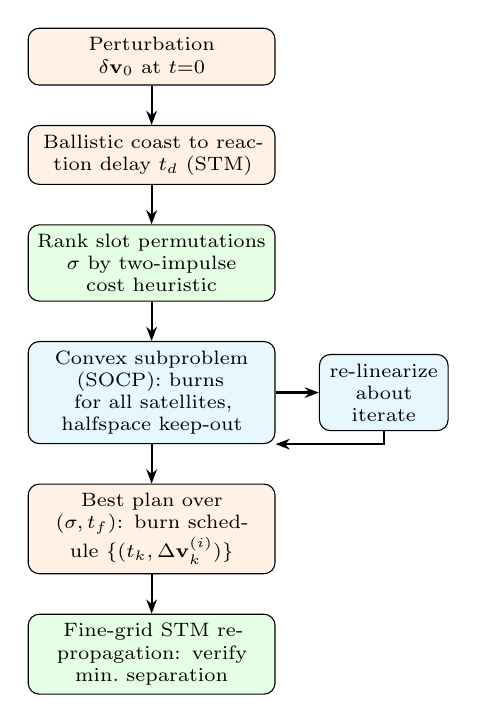
\begin{tikzpicture}[
    node distance=0.38cm,
    block/.style={rectangle, draw, rounded corners, fill=orange!10,
                  minimum height=0.62cm, minimum width=2.9cm,
                  text width=2.9cm, align=center, font=\scriptsize},
    dblock/.style={rectangle, draw, rounded corners, fill=cyan!10,
                  minimum height=0.62cm, minimum width=2.9cm,
                  text width=2.9cm, align=center, font=\scriptsize},
    gblock/.style={rectangle, draw, rounded corners, fill=green!10,
                  minimum height=0.62cm, minimum width=2.9cm,
                  text width=2.9cm, align=center, font=\scriptsize},
    arr/.style={-{Stealth[length=1.8mm]}, thick},
]
\node[block] (pert) {Perturbation $\delta\mathbf{v}_0$ at $t{=}0$};
\node[block, below=0.5cm of pert] (coast) {Ballistic coast to reaction delay $t_d$ (STM)};
\node[gblock, below=0.5cm of coast] (assign) {Rank slot permutations $\sigma$ by two-impulse cost heuristic};
\node[dblock, below=0.5cm of assign] (socp) {Convex subproblem (SOCP): burns for all satellites, halfspace keep-out};
\node[dblock, right=0.55cm of socp, text width=1.4cm, minimum width=1.4cm] (relin) {re-linearize about iterate};
\node[block, below=0.5cm of socp] (plan) {Best plan over $(\sigma, t_f)$: burn schedule $\{(t_k, \Delta\mathbf{v}^{(i)}_k)\}$};
\node[gblock, below=0.5cm of plan] (verify) {Fine-grid STM re-propagation: verify min.\ separation};

\draw[arr] (pert) -- (coast);
\draw[arr] (coast) -- (assign);
\draw[arr] (assign) -- (socp);
\draw[arr] (socp.east) -- (relin.west);
\draw[arr] (relin.south) |- (socp.south east);
\draw[arr] (socp) -- (plan);
\draw[arr] (plan) -- (verify);
\end{tikzpicture}%
}
\caption{SCP recovery pipeline. The exact CW STM propagates the uncontrolled
coast; slot permutations are ranked by a closed-form heuristic; each candidate
assignment is solved as a sequence of SOCPs whose only linearized element is
the keep-out constraint, imposed at densely sub-sampled times along every
coast segment; the winning plan is re-propagated on a fine grid to confirm
the realized minimum separation.}
\label{fig:pipeline}
\end{figure}

Figure~\ref{fig:pipeline} summarizes the planner. We discretize the controlled
window $[t_d, t_f]$ into $N$ steps of length $\Delta t$ and allow an impulse
$\Delta\mathbf{v}^{(i)}_k$ for every satellite $i$ at every node $k = 0,\dots,N$
(``burn as many times as necessary''). Burn \emph{times} on a grid are the
convex surrogate for continuous burn-time optimization, which is non-convex
(the burn time enters the STM nonlinearly); as $\Delta t \to 0$ the grid
solution approaches the continuous impulsive optimum, and the group-lasso
objective below keeps the selected burn set finite and sparse regardless of
grid density. Path constraints, by contrast, \emph{are} imposed continuously
in time (sub-sampled between nodes), as described below. For a fixed slot
assignment $\sigma$ and recovery time $t_f$, the subproblem is
\begin{align}
\label{eq:scp}
\min_{\Delta\mathbf{v}, \mathbf{x}, s, m} \;
& \sum_{i}\sum_{k} \bigl\|\Delta\mathbf{v}^{(i)}_k\bigr\|_2
  + w_{\mathrm{bal}}\, m
  + w_{s} \textstyle\sum s \\
\text{s.t.}\;\;
& \mathbf{x}^{(i)}_{k+1} = \Phi(\Delta t)\bigl(\mathbf{x}^{(i)}_k + B\,\Delta\mathbf{v}^{(i)}_k\bigr), \nonumber\\
& \mathbf{x}^{(i)}_N + B\,\Delta\mathbf{v}^{(i)}_N = \mathbf{x}_{\mathrm{slot},\sigma(i)}, \nonumber\\
& \bigl\|\Delta\mathbf{v}^{(i)}_k\bigr\|_2 \le \Delta v_{\max}, \quad
  \textstyle\sum_k \bigl\|\Delta\mathbf{v}^{(i)}_k\bigr\|_2 \le \min(v_{\mathrm{fuel}},\, m), \nonumber\\
& \hat{\mathbf{n}}^{ij}(\tau)^{\top}\bigl(\mathbf{r}^{(i)}(\tau) - \mathbf{r}^{(j)}(\tau)\bigr) \ge d_{\min} + \epsilon - s^{ij}(\tau), \nonumber\\
& \qquad s^{ij}(\tau) \ge 0 \quad \forall\, i<j,\;\; \tau \in \mathcal{T}_c, \nonumber
\end{align}
where $m$ is an epigraph variable for the maximum per-satellite fuel use. The
objective combines three terms. The sum of $\ell_2$ impulse norms is the total
constellation $\Delta v$; as a group lasso it drives most candidate impulses to
exactly zero, so the solver \emph{selects} the number of burns. The balancing
term $w_{\mathrm{bal}}\,m$ penalizes concentrating fuel use on one vehicle,
since mission life ends when the first satellite exhausts its budget. The
slack penalty $w_s \sum s$ is an exact penalty that preserves subproblem
feasibility during early iterations. Time of flight enters through an outer
search: candidate $t_f$ values are each solved and compared by
$J = \Delta v_{\mathrm{tot}} + w_{t_f} t_f$, trading fuel against time out of
formation.

\textbf{Continuous-time collision enforcement:} The coasting state between
burn nodes is $\mathbf{x}(t_k + \tau) = \Phi(\tau)\bigl(\mathbf{x}_k +
B\,\Delta\mathbf{v}_k\bigr)$, which is \emph{affine} in the decision
variables, so the keep-out constraint can be imposed at arbitrary times
without changing the problem class. We impose it on the dense sample set
$\mathcal{T}_c$, every $\Delta t / 6$ along every coast segment (exact STM
interpolation, no added burn nodes), with a margin $\epsilon = 10$\,m padding
$d_{\min}$ against the residual excursion between adjacent samples. The
trajectory therefore cannot pass through a keep-out sphere between burn
nodes, and a fine-grid STM re-propagation of the executed plan confirms the
realized minimum separation.

\textbf{Linearization:} The CW dynamics in \eqref{eq:scp} are \emph{exactly}
linear, so the pairwise keep-out constraint is the only non-convexity. At
each constraint time $\tau$, the previous iterate supplies the relative
(line-of-sight) position $\bar{\mathbf{p}}^{ij}(\tau) =
\bar{\mathbf{r}}^{(i)}(\tau) - \bar{\mathbf{r}}^{(j)}(\tau)$, and we
constrain the new iterate to the supporting halfspace of the keep-out sphere
with normal $\hat{\mathbf{n}}^{ij}(\tau) = \bar{\mathbf{p}}^{ij}(\tau) /
\|\bar{\mathbf{p}}^{ij}(\tau)\|_2$---the hyperplane tangent to the sphere
where the line of sight exits it, perpendicular to that line of sight. This
halfspace is entirely \emph{outside} the sphere, so the linearization is a
conservative inner approximation of the true feasible set: every iterate
satisfying it is collision-free at every imposed sample, and no trust region
is needed for constraint validity~\cite{morgan2014,mao2016}. Iteration
re-aims the halfspace normal to recover optimality; we iterate from a
ballistic reference until the total $\Delta v$ changes by less than
$10^{-3}$\,m/s.

\textbf{Slot assignment:} Any permutation $\sigma$ of the satellites over the
original slots restores the required spacing. We rank all $n!$ permutations by
the summed closed-form two-impulse cost \eqref{eq:twoimpulse} of sending each
satellite to its candidate slot, then solve \eqref{eq:scp} exactly for the
best few. For $n{=}3$ this heuristic-plus-exact search adds negligible cost.

\subsection{Codebase}

All components are implemented in our Python package \texttt{cwsim}: the STM
and propagation (\texttt{dynamics}), analytic chief orbit and RIC/ECI frames
(\texttt{orbits}, \texttt{frames}), formation containers
(\texttt{satellites}), the simulation driver (\texttt{simulation}), the SCP
planner and baseline (\texttt{scp}), and a dual-frame interactive 3D
visualization with a textured Earth (\texttt{visualization}, built on
PyVista~\cite{sullivan2019}). Convex subproblems are modeled in
CVXPY~\cite{diamond2016} and solved with Clarabel~\cite{clarabel2024}. The
project proposal targeted MATLAB; we moved to Python for the open-source
conic-solver and 3D-rendering ecosystem.

\section{Simulation Setup and Verification}
\label{sec:setup}

\textbf{Scenario:} Three homogeneous satellites in an equally spaced
along-track formation ($\pm1$\,km) about a circular 550\,km, $51.6^\circ$
chief orbit (period $95.6$\,min). At $t{=}0$ the middle satellite (Sat-2)
receives an unexpected $\delta\mathbf{v}_0$; no corrective burns are allowed
until the reaction delay $t_d$. Table~\ref{tab:params} lists the scenario and
solver settings. We assume CW dynamics, perfect noise-free state knowledge,
and perfect impulsive execution, per the project problem statement.

\begin{table}[t]
\centering
\caption{Scenario and Solver Settings.}
\label{tab:params}
\small
\begin{tabular}{@{}ll@{}}
\toprule
\textbf{Parameter} & \textbf{Setting} \\
\midrule
Chief orbit & circular, $h_0 = 550$\,km, $i = 51.6^\circ$ \\
Orbit period $T$ & $95.6$\,min; $n = \sqrt{\mu/a_0^3}$ \\
Formation & 3 satellites, $\pm1$\,km along-track \\
Keep-out radius $d_{\min}$ & $200$\,m (pairwise) \\
Keep-out sampling $\mathcal{T}_c$ & every $\Delta t/6$ (STM interpolation) \\
Collision margin $\epsilon$ & $10$\,m pad on $d_{\min}$ \\
Per-burn limit $\Delta v_{\max}$ & $0.5$\,m/s \\
Fuel budget $v_{\mathrm{fuel}}$ & $5$\,m/s per satellite \\
Burn grid $\Delta t$ & $150$\,s (sweep); $90$\,s (demo) \\
Balance weight $w_{\mathrm{bal}}$ & $0.1$ \\
Slack penalty $w_s$ & $1$\,(m/s)/m (exact penalty) \\
Time weight $w_{t_f}$ & $2\times10^{-5}$\,(m/s)/s (demo) \\
SCP convergence & $|\Delta(\Delta v_{\mathrm{tot}})| < 10^{-3}$\,m/s \\
Assignments solved & best 2--3 of $3!$ (heuristic-ranked) \\
Solver & CVXPY + Clarabel (SOCP) \\
Recovery time $t_f$ & $2.15\,T$ (sweep); traded (demo) \\
\bottomrule
\end{tabular}
\end{table}

\textbf{Verification:} Because every downstream result rests on the STM, we
verify the dynamics stack directly (Table~\ref{tab:verification}): the STM
matches RK4 integration of \eqref{eq:cw} at the $10^{-12}$\,m level over 1.5
orbits, satisfies the semigroup property
$\Phi(t_1{+}t_2) = \Phi(t_2)\Phi(t_1)$ and $\Phi(0) = I$, the two-impulse law
\eqref{eq:twoimpulse} achieves its target to machine precision, the
RIC$\leftrightarrow$ECI mapping round-trips exactly, and the along-track
offset equilibrium is preserved.

\begin{table}[t]
\centering
\caption{Numerical verification of the dynamics stack.}
\label{tab:verification}
\small
\begin{tabular}{@{}lc@{}}
\toprule
\textbf{Check} & \textbf{Max error} \\
\midrule
STM vs.\ RK4 ($1.5$ orbits), position & $4.1\times10^{-12}$\,m \\
STM semigroup $\Phi(t_1{+}t_2) = \Phi(t_2)\Phi(t_1)$ & machine precision \\
Two-impulse arrival position error & $7.1\times10^{-15}$\,m \\
RIC $\leftrightarrow$ ECI round-trip & $<10^{-9}$ (all states) \\
Along-track equilibrium drift ($5000$\,s) & $<10^{-9}$\,m \\
\bottomrule
\end{tabular}
\end{table}

\section{Experiments, Results, and Discussion}
\label{sec:experiments}

\textbf{Metrics:} We report total constellation $\Delta v$ (sum of all
impulse magnitudes over all satellites), the chosen slot assignment, the
number of burns the group-lasso objective selects, and the fine-grid minimum
pairwise separation over the full window $[0, t_f]$, including the
uncontrolled delay. Both architectures are evaluated at identical $(t_d, t_f)$
for a fair comparison.

\textbf{Headline scenario:} For $\delta\mathbf{v}_0 = [0.05, 0.10,
0.03]$\,m/s on Sat-2 and $t_d = 0.25\,T$, the baseline returns Sat-2 to its
slot for $2.27$\,m/s. The SCP planner instead swaps Sat-1 and Sat-2
(Fig.~\ref{fig:highlight}) for a total of $0.30$\,m/s---an $87\%$
reduction---splitting the effort $0.12$/$0.18$\,m/s between the two movers
while Sat-3 holds station, with $379$\,m minimum separation against the
$200$\,m keep-out. With the time weight active, the outer search also selects
the shortest candidate recovery time, since the fuel saved by waiting longer
was smaller than the time penalty.

\begin{table*}[t]
\centering
\caption{Total constellation $\Delta v$ [m/s] vs.\ reaction delay
($|\delta\mathbf{v}_0| = 0.1$\,m/s, $t_f = 2.15\,T$). Parenthesized
superscript $^{\mathrm{sw}}$ marks SCP solutions that chose to re-slot
(swap Sat-1$\leftrightarrow$Sat-2). The baseline maneuvers only Sat-2.}
\label{tab:delay}
\small
\setlength{\tabcolsep}{6pt}
\begin{tabular}{@{}llcccc@{}}
\toprule
\textbf{Perturbation} & \textbf{Method} & $t_d = 0.1\,T$ & $t_d = 0.25\,T$ & $t_d = 0.5\,T$ & $t_d = 1.0\,T$ \\
\midrule
Radial      & Baseline & 0.452 & 0.308 & 0.102 & 0.100 \\
            & SCP      & \textbf{0.050} & \textbf{0.050} & \textbf{0.050} & \textbf{0.056} \\
\midrule
Along-track & Baseline & 0.379 & 0.464 & 0.695 & 0.387 \\
            & SCP      & \textbf{0.167}$^{\mathrm{sw}}$ & \textbf{0.205}$^{\mathrm{sw}}$ & \textbf{0.270}$^{\mathrm{sw}}$ & \textbf{0.299}$^{\mathrm{sw}}$ \\
\midrule
Cross-track & Baseline & 0.452 & 0.308 & 0.100 & 0.100 \\
            & SCP      & \textbf{0.100} & \textbf{0.100} & \textbf{0.100} & \textbf{0.100} \\
\bottomrule
\end{tabular}
\end{table*}

\begin{table}[t]
\centering
\caption{Total constellation $\Delta v$ [m/s] vs.\ perturbation magnitude
($t_d = 0.25\,T$, $t_f = 2.15\,T$).}
\label{tab:magnitude}
\small
\setlength{\tabcolsep}{4.5pt}
\begin{tabular}{@{}llccc@{}}
\toprule
\textbf{Perturbation} & \textbf{Method} & $0.05$\,m/s & $0.1$\,m/s & $0.2$\,m/s \\
\midrule
Radial      & Baseline & 0.154 & 0.308 & 0.616 \\
            & SCP      & \textbf{0.025} & \textbf{0.050} & \textbf{0.100} \\
\midrule
Along-track & Baseline & 0.232 & 0.464 & 0.928 \\
            & SCP      & \textbf{0.162}$^{\mathrm{sw}}$ & \textbf{0.205}$^{\mathrm{sw}}$ & \textbf{0.409}$^{\mathrm{sw}}$ \\
\midrule
Cross-track & Baseline & 0.154 & 0.308 & 0.616 \\
            & SCP      & \textbf{0.050} & \textbf{0.100} & \textbf{0.200} \\
\bottomrule
\end{tabular}
\end{table}

\begin{figure*}[t]
\centering
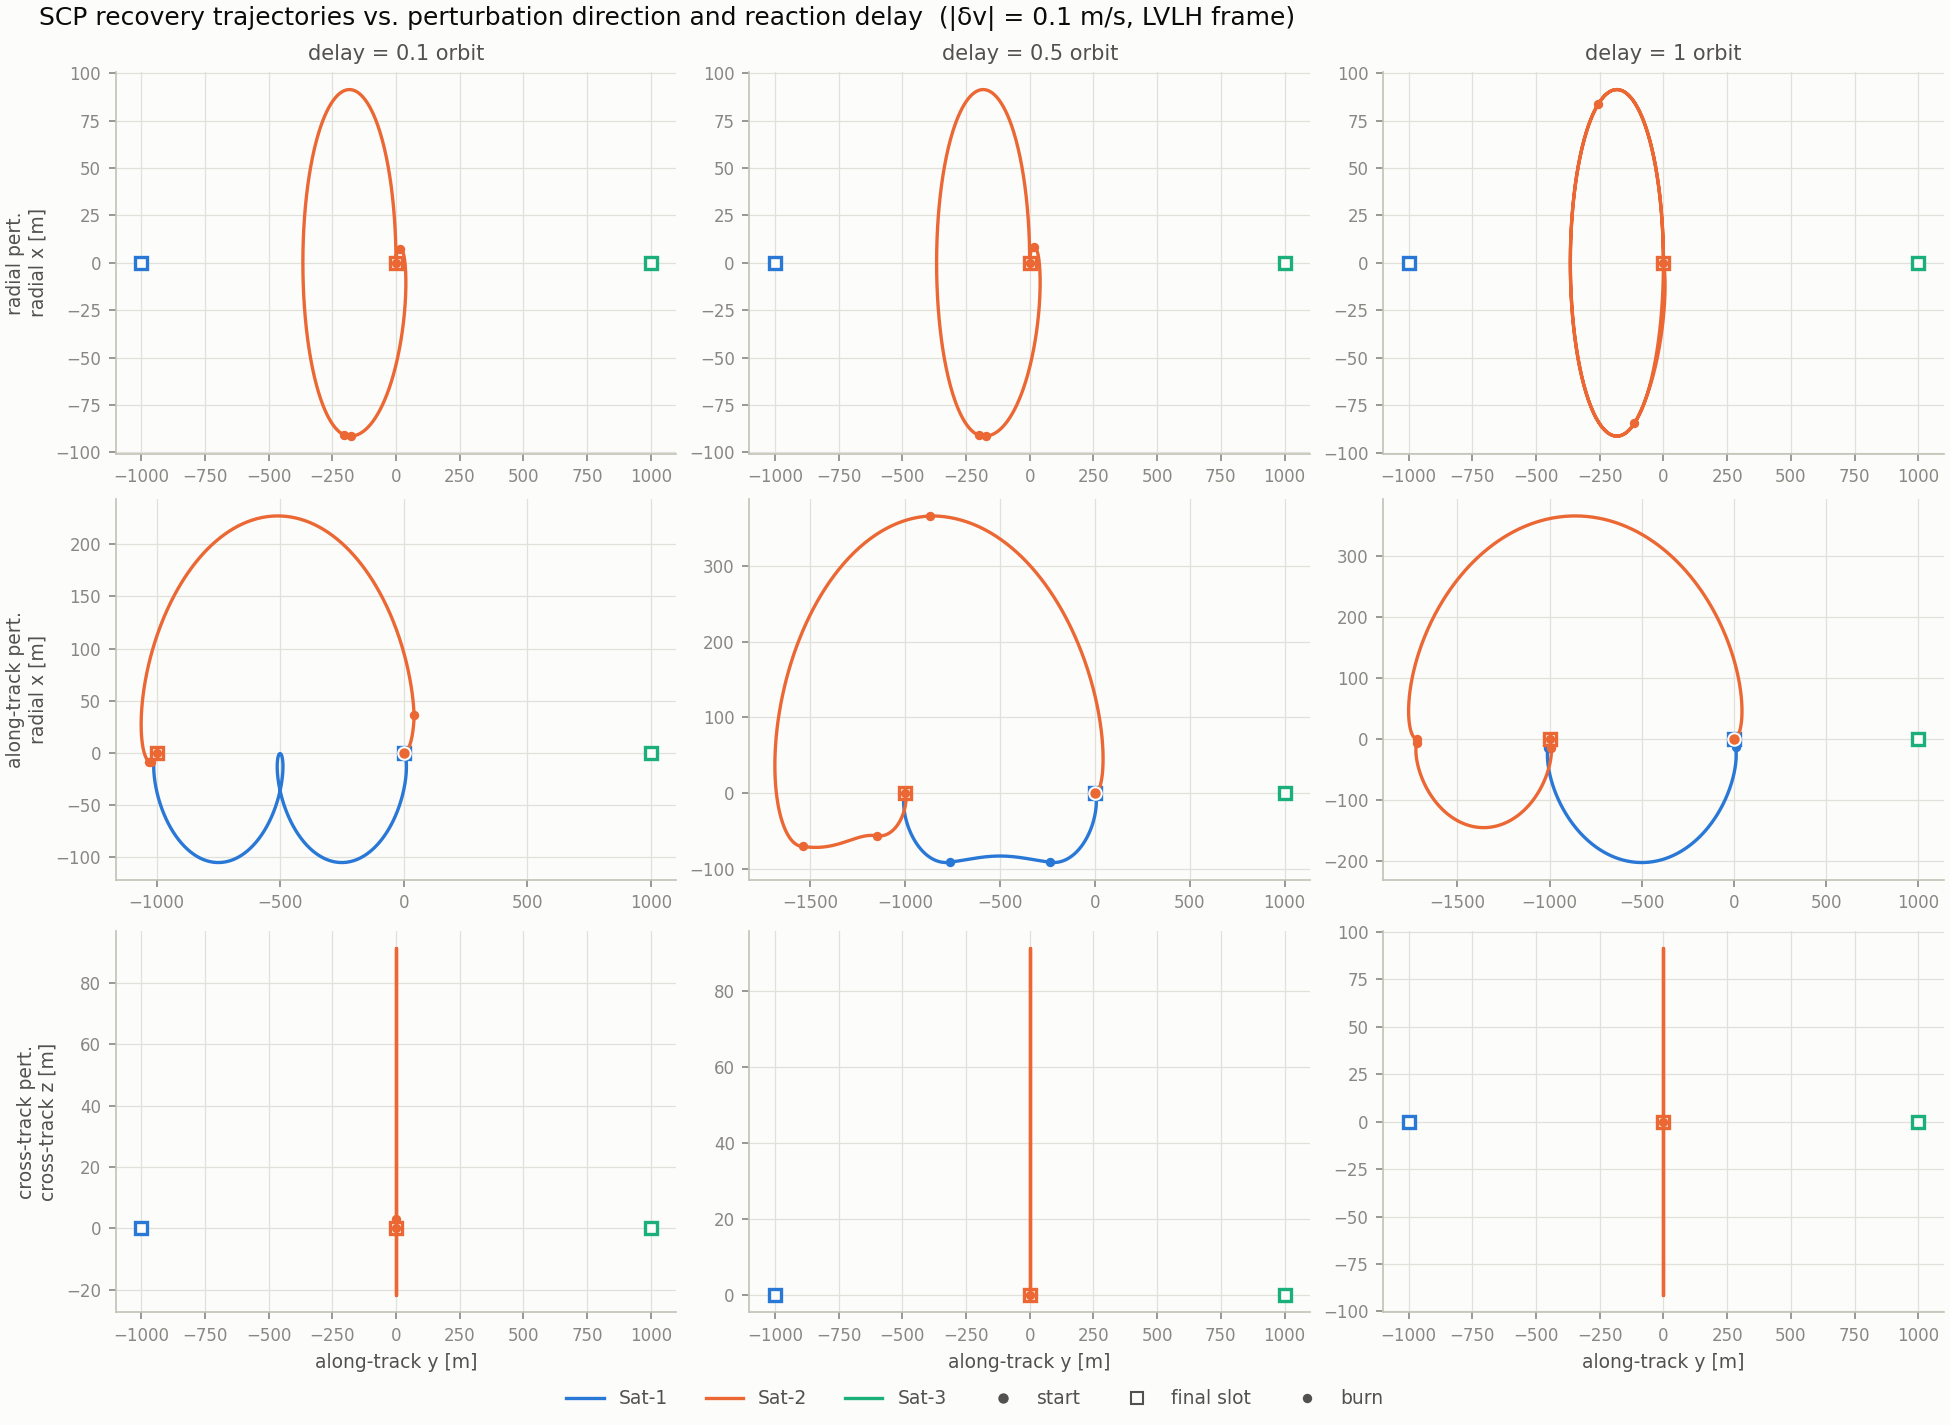
\includegraphics[width=\linewidth]{figures/sweep_trajectories.png}
\caption{SCP recovery trajectories in the RIC frame as the perturbation
direction (rows) and reaction delay (columns) vary, at
$|\delta\mathbf{v}_0| = 0.1$\,m/s. Radial perturbations (top) produce a
bounded $2{\times}1$ in-plane ellipse that the planner closes for
$\approx|\delta v|/2$. Along-track perturbations (middle) accumulate secular
drift that grows with delay; in every case the planner swaps Sat-2 (orange)
with Sat-1 (blue) rather than reversing the drift, and at longer delays Sat-1
flies a cooperative transfer to the vacated center slot. Cross-track
perturbations (bottom) excite a decoupled out-of-plane oscillation cancelled
for exactly $|\delta v|$.}
\label{fig:trajectories}
\end{figure*}

\begin{figure}[t]
\centering
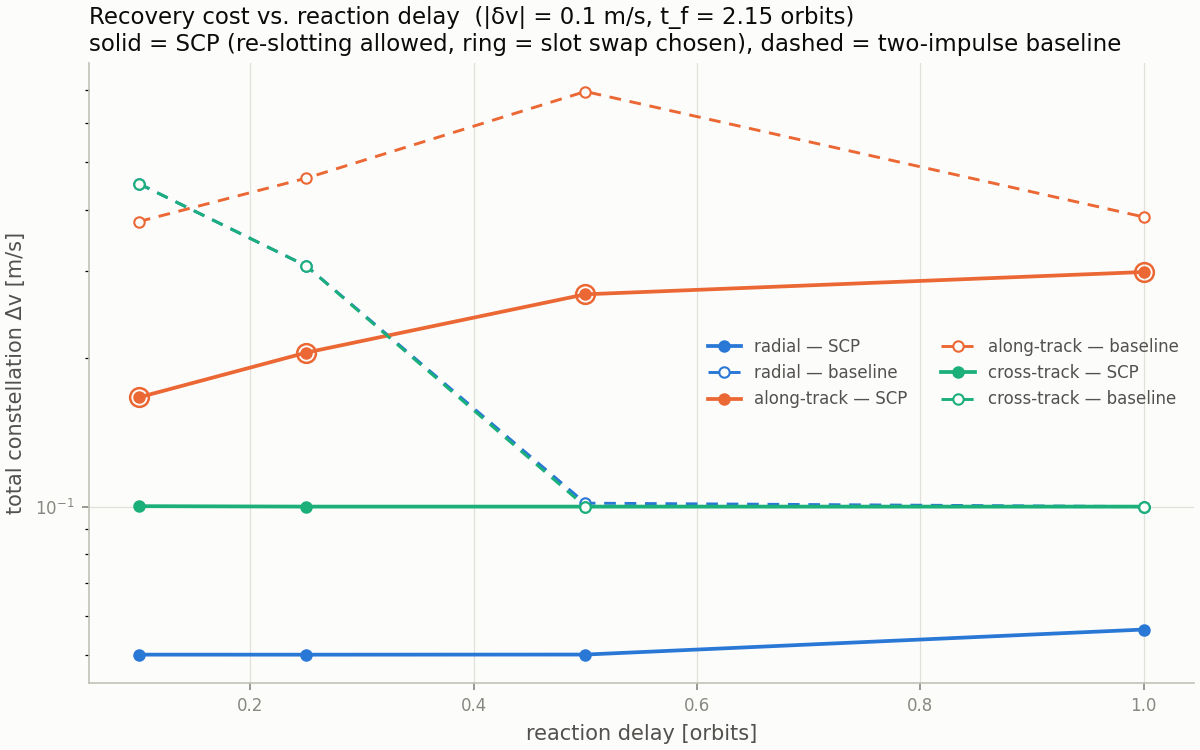
\includegraphics[width=\columnwidth]{figures/sweep_cost_vs_delay.png}
\caption{Total constellation $\Delta v$ vs.\ reaction delay
($|\delta\mathbf{v}_0| = 0.1$\,m/s, log scale). Solid: SCP (ring = slot swap
chosen); dashed: two-impulse baseline. SCP cost is flat in delay for the
bounded radial and cross-track responses, and grows slowly for along-track,
while the phase-locked baseline varies strongly with burn timing.}
\label{fig:cost_delay}
\end{figure}

\begin{figure}[t]
\centering
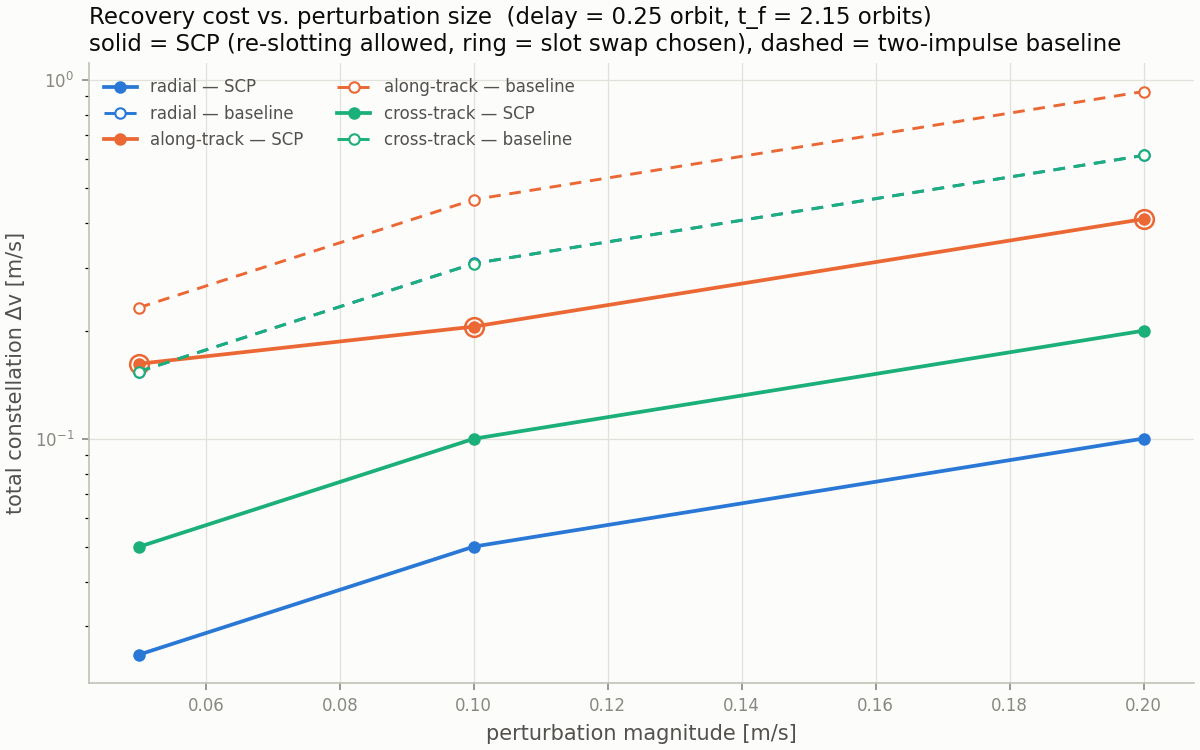
\includegraphics[width=\columnwidth]{figures/sweep_cost_vs_magnitude.png}
\caption{Total constellation $\Delta v$ vs.\ perturbation magnitude
($t_d = 0.25\,T$, log scale). Costs scale essentially linearly with
$|\delta\mathbf{v}_0|$ for both methods; SCP maintains a $1.5$--$6\times$
advantage across the range.}
\label{fig:cost_mag}
\end{figure}

\noindent \textbf{Trade study:} Tables~\ref{tab:delay} and~\ref{tab:magnitude}
and Figures~\ref{fig:trajectories}--\ref{fig:cost_mag} sweep the perturbation
direction and magnitude and the reaction delay at fixed $t_f = 2.15\,T$
(chosen so that no swept horizon $t_f - t_d$ lands on a half-period multiple,
where the baseline diverges; see Sec.~\ref{sec:baseline}).

\subsection{Analysis and discussion}
\label{sec:discussion}

We organize the analysis by perturbation direction, since the CW dynamics
decouple the three channels into qualitatively different responses, then
discuss the delay trade, collision safety, and solver behavior.

\paragraph{Along-track: re-slotting always wins.}
An along-track $\delta v$ changes the effective semi-major axis and produces
secular drift---the expensive, dangerous channel, and the core of the
project's hypothesis. In \emph{every} along-track case in
Tables~\ref{tab:delay} and~\ref{tab:magnitude}, the SCP planner chooses to
swap Sat-2 with the neighbor it is drifting toward rather than reverse the
drift, cutting cost by $23$--$61\%$ (e.g.\ $0.270$ vs.\ $0.695$\,m/s at
$t_d = 0.5\,T$; the smallest margin, $23\%$, occurs at the one-orbit delay,
where the accumulated drift has made even the swap expensive). The mechanism is visible in
Figure~\ref{fig:trajectories} (middle row): Sat-2 rides its natural drift
loop into the adjacent slot while Sat-1 flies a short cooperative transfer to
the vacated center---two cheap maneuvers aligned with the dynamics instead of
one expensive maneuver against them. This directly answers the project
question: when the perturbation is along-track, leveraging the drift through
re-ordering is uniformly cheaper than restoring the original slot order.

\paragraph{Radial: recovery at half the perturbation.}
A radial $\delta v$ excites the bounded $2{\times}1$ relative ellipse with no
secular term. The SCP cost is $\approx|\delta v|/2$ at every delay
(e.g.\ $0.050$ for a $0.100$\,m/s kick): with freely chosen burn times the
planner cancels the oscillation at a favorable phase, exploiting the
$2{\times}$ along-track-to-radial control authority of the Coriolis coupling.
The baseline, whose burn times are pinned to $t_d$ and $t_f$, pays up to
$9\times$ more when those times land at unfavorable phases ($0.452$ at
$t_d = 0.1\,T$) and only approaches the SCP cost when the delay happens to
align the phase.

\paragraph{Cross-track: cost exactly $|\delta v|$.}
The out-of-plane channel is a decoupled harmonic oscillator, so the minimum
recovery cost is exactly the perturbation magnitude---cancel the oscillation
at a node crossing---and the SCP solution achieves $0.100$\,m/s at every
delay, usually with a single burn. The phase-locked baseline again pays up to
$4.5\times$ more at short delays. Neither radial nor cross-track cases ever
trigger re-slotting: the responses are bounded, so there is no drift to
exploit.

\paragraph{Reaction delay.}
Delay matters only where drift accumulates. Along-track SCP cost grows from
$0.167$ to $0.299$\,m/s as the delay grows from $0.1\,T$ to $1.0\,T$---waiting
is strictly costly when the satellite is drifting away---while radial and
cross-track costs are essentially flat because the uncontrolled motion is
bounded. The baseline's non-monotone delay dependence is dominated by burn
phasing rather than by the physics of the perturbation, a further argument
for burn-time-free planning.

\paragraph{Collision safety.}
The keep-out constraint is active, not decorative: the along-track drift
carries Sat-2 directly through Sat-1's position. The baseline, with no
collision logic, dips to $192.6$\,m minimum separation in one swept
case---inside the $200$\,m keep-out. With the keep-out imposed at every
$\Delta t/6$ along each coast segment plus the $10$\,m margin, every SCP
plan's fine-grid minimum separation stays strictly outside the sphere
($\geq 210.6$\,m across the sweep); the one case where the constraint binds
pays only $0.003$\,m/s more than node-only enforcement did.

\paragraph{Solver behavior.}
Across the sweep, subproblems solve in seconds and the SCP loop converges in
$2$ iterations when the ballistic reference is already collision-feasible,
and in $6$--$8$ iterations when the initial halfspace linearization forces a
large detour that subsequent re-linearizations relax. The exact-penalty slack
is nonzero only on the first iteration of hard cases and returns to zero
thereafter, consistent with the conservative inner approximation guaranteeing
feasible iterates. The group-lasso objective selects $2$--$9$ burns per plan
without any integer variables.

\subsection{Limitations}

Our conclusions inherit the CW assumptions: linearized relative dynamics about
a circular chief, no $J_2$, drag, or navigation and execution errors, and
impulsive burns whose times live on a dense grid (continuous burn-time
optimization is non-convex; the grid solution approaches it as
$\Delta t \to 0$). The keep-out constraint is sampled densely in time with a
margin rather than imposed exactly over continuous intervals, and is
non-convex, so SCP returns locally optimal plans with no global
certificate---the assignment search mitigates, but does not eliminate, this. The slot-assignment heuristic
could in principle rank the true optimum below the permutations solved
exactly, and the study covers a three-satellite formation; the formulation
scales to $n$ satellites, but the $n!$ assignment enumeration would need
replacement (e.g.\ by a linear assignment relaxation) for large $n$.

\section{Conclusion and Future Work}
\label{sec:conclusion}

We presented \texttt{cwsim}, a modular CW formation-flying simulator built on
the exact closed-form 3-DOF STM, and used it to compare two recovery
architectures for a perturbed three-satellite along-track formation: a
closed-form two-impulse return-to-slot baseline and an SCP planner that
coordinates burns across all satellites with re-slotting, keep-out spheres,
thrust limits, fuel budgets, and fuel balancing. Across perturbation
directions, magnitudes, and reaction delays, SCP reduces total constellation
$\Delta v$ by up to $89\%$ (median ${\approx}56\%$); for along-track
perturbations the optimizer always
re-slots, confirming the project hypothesis that the natural drift should be
leveraged rather than reversed. The study also surfaced two practical
warnings for operators: the two-impulse law diverges near half-period
transfer horizons, and without explicit collision constraints it can violate
keep-out margins that the convex planner honors by construction.

Future work includes validating the plans against nonlinear two-body and
$J_2$-perturbed dynamics, formal continuous-interval collision certificates
(bounding the excursion between constraint samples), Monte Carlo
robustness under navigation and execution errors, larger constellations with
relaxation-based assignment, and a receding-horizon variant that replans as
tracking errors accumulate.

\section*{Contributions and Acknowledgements}

% TODO: update each member's contribution list.
\textbf{Rahul Ayanampudi:} CW dynamics and STM implementation, two-impulse
baseline, SCP formulation and implementation, trade-study design, simulator
and visualization, report writing.\\

\textbf{Zeb Barry:} % TODO: fill in contributions.
\\

\textbf{Julian Brown:} % TODO: fill in contributions.
\\

\textbf{Generative AI usage.} We used AI tools to supplement portions of this
work. AI assisted with generating the initial codebase scaffolding for the
simulator, visualization, and solver modules, and with LaTeX table and figure
formatting. We maintained oversight of the formulation and verified the
dynamics stack against independent numerical integration
(Table~\ref{tab:verification}); all problem definitions, parameter choices,
reported metrics, and conclusions were reviewed and verified by us.

\balance
{\small
\begin{thebibliography}{99}

\bibitem{cw1960}
W.~H. Clohessy and R.~S. Wiltshire.
Terminal guidance system for satellite rendezvous.
\emph{Journal of the Aerospace Sciences}, 27(9):653--658, 1960.

\bibitem{hill1878}
G.~W. Hill.
Researches in the lunar theory.
\emph{American Journal of Mathematics}, 1(1):5--26, 1878.

\bibitem{vallado2013}
D.~A. Vallado.
\emph{Fundamentals of Astrodynamics and Applications}.
Microcosm Press, 4th edition, 2013.

\bibitem{schaub2018}
H.~Schaub and J.~L. Junkins.
\emph{Analytical Mechanics of Space Systems}.
AIAA Education Series, 4th edition, 2018.

\bibitem{alfriend2010}
K.~T. Alfriend, S.~R. Vadali, P.~Gurfil, J.~P. How, and L.~Breger.
\emph{Spacecraft Formation Flying: Dynamics, Control and Navigation}.
Elsevier, 2010.

\bibitem{nasa_starling}
NASA Ames Research Center.
Starling: Swarm satellite technology demonstration.
\url{https://www.nasa.gov/mission/starling/}, 2023.

\bibitem{acikmese2007}
B.~A\c{c}{\i}kme\c{s}e and S.~R. Ploen.
Convex programming approach to powered descent guidance for Mars landing.
\emph{Journal of Guidance, Control, and Dynamics}, 30(5):1353--1366, 2007.

\bibitem{lu2013}
P.~Lu and X.~Liu.
Autonomous trajectory planning for rendezvous and proximity operations by
conic optimization.
\emph{Journal of Guidance, Control, and Dynamics}, 36(2):375--389, 2013.

\bibitem{morgan2014}
D.~Morgan, S.-J. Chung, and F.~Y. Hadaegh.
Model predictive control of swarms of spacecraft using sequential convex
programming.
\emph{Journal of Guidance, Control, and Dynamics}, 37(6):1725--1740, 2014.

\bibitem{mao2016}
Y.~Mao, M.~Szmuk, and B.~A\c{c}{\i}kme\c{s}e.
Successive convexification of non-convex optimal control problems and its
convergence properties.
In \emph{IEEE Conference on Decision and Control}, pages 3636--3641, 2016.

\bibitem{boyd2004}
S.~Boyd and L.~Vandenberghe.
\emph{Convex Optimization}.
Cambridge University Press, 2004.

\bibitem{diamond2016}
S.~Diamond and S.~Boyd.
{CVXPY}: A {Python}-embedded modeling language for convex optimization.
\emph{Journal of Machine Learning Research}, 17(83):1--5, 2016.

\bibitem{clarabel2024}
P.~J. Goulart and Y.~Chen.
Clarabel: An interior-point solver for conic programs with quadratic
objectives.
\emph{arXiv preprint arXiv:2405.12762}, 2024.

\bibitem{sullivan2019}
C.~B. Sullivan and A.~Kaszynski.
{PyVista}: 3D plotting and mesh analysis through a streamlined interface for
the Visualization Toolkit ({VTK}).
\emph{Journal of Open Source Software}, 4(37):1450, 2019.

\end{thebibliography}
}

\end{document}
